%Works on MiKTeX only
%hint by http://goemonx.blogspot.de/2012/01/pdflatex-ligaturen-und-copynpaste.html
%also http://tex.stackexchange.com/questions/4397/make-ligatures-in-linux-libertine-copyable-and-searchable
%This allows a copy'n'paste of the text from the paper
\input glyphtounicode.tex
\pdfgentounicode=1

In the past years, organizations have seen changes in the field of software development when it comes to implementation models and related processes. Constant changes, especially in requirements become difficult when more rigid software processes are applied. Slowness to accommodate uncertainty and rapid changes inevitably lead to obsolescence of software and customer dissatisfaction \cite{agile:1}. Changes in requirements may turn software artifacts already planned, designed, specified and even already implemented in obsolete and outdated artifacts.
It is desirable that software processes have sufficient flexibility to accommodate inevitable changes and uncertainties. At the same time, it is expectable that these processes might be described, monitored and improved.
For that reason one of the most important approaches for software development in the last years is the use of development methodologies. 

There are two types of methodologies: Waterfall and Agile. The Waterfall method is one of the oldest product development models. The success of the model in delivering a robust, high quality product has been well documented. Agile methods were developed to overcome the limitations of traditional software development methods such waterfall method.

This section describes the best methodology approaches for software development including their benefits and challenges when applied to different scenarios. 

\subsection{Waterfall Methodology}

Waterfall is a sequential model where the software development lifecycle is divided into 5 phases: (1) Requirement Analysis, (2) Design (3) Implementation (4) Verification (5) Maintenance, with each phase having its own tasks and goals. 

\begin{figure}[h]
    \centering
    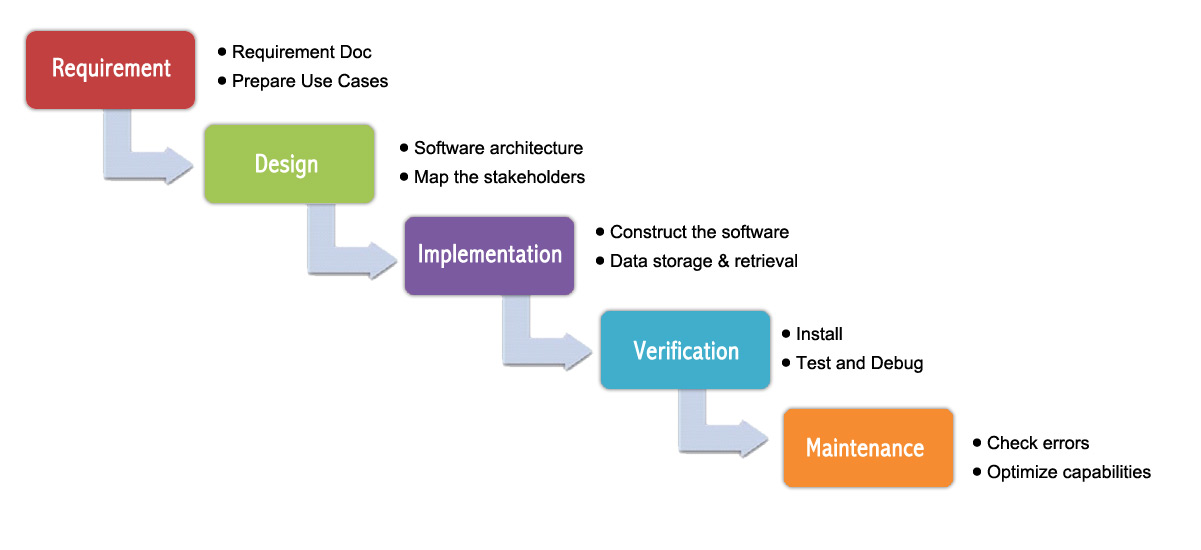
\includegraphics[width=\textwidth]{Waterfall}
    \caption{Waterfall Process Model}
    \label{fig:waterfall}
\end{figure}

As this process is sequential, once a step has been completed, developers can’t go back to a previous step – not without scratching the whole project and starting from the beginning. There is no place for change or error, so a project outcome and an extensive plan must be set in the beginning and then followed carefully, and for that reason overlapping is typically impossible in this methodology.
In waterfall methodologies all the requirements gathering and design work is done before any coding takes place.
 
Despite the success of the model in large and complex projects, it has a number of drawbacks like inflexibility, huge processes and the associated documentations irrespective of the size of the project \cite{method:Tommy2016}. A brief description of the advantages and disadvantages of this methodology is given bellow:\\

\textbf{Advantages of the Waterfall Methodology}
\begin{itemize}

\item Potential issues that would have been found during development can be researched and treated during the design phase, meaning that an alternate solution is selected before any code is written. Developers and customers agree on what will be delivered early in the development lifecycle making planning and designing more straightforward.\\

\item The development process tends to be better documented due to the fact that this methodology places greater emphasis on documentation, like requirements and design documents, being useful for many organizations.\\

\item The software can be designed completely and more carefully, based on a more complete understanding of all software deliverables. This provides a better software design with less likelihood of the “piecemeal effect”, a development phenomenon that can occur as pieces of code are defined and subsequently added to an application without knowing if they may or may not fit well \cite{waterfall:piecemeal}.
\end{itemize}

\textbf{Disadvantages of the Waterfall Methodology}
\begin{itemize}
\item If a set of change requests are introduced into the product while is undergoing testing, pausing the testing phase to do development is extremely heavy and expensive. So going back to a previous phase of the product's lifecycle is always a challenge.\\

\item It is not the best approach for large and complicated projects, where requirements may be frequently in change.\\

\item Since testing is one of the last phases in waterfall methodology, identifying risks and challenges in the earlier phases, and preparing a risk mitigation strategy, always become challenging.\\

\end{itemize}

\subsection{Agile Methodology}
Agile methodologies were developed to overcome the limitations of the Waterfall methodology. Instead of extensive planning and design up front, agile follows an incremental and iterative approach to development, where requirements and solutions evolve through collaboration between self-organizing, cross-functional teams - incorporating planners, designers, developers and testers - and customer. The Agile development refers to any development process that is aligned with the concepts of Agile Manifesto that says \cite{agile:manifesto}:\\

\textit{"We are uncovering better ways of developing software by doing it and helping others do it. We value:}

\begin{itemize}
\item \textit{Individuals and interactions over processes and tools.}
\item \textit{Working software over comprehensive documentation.}
\item \textit{Customer collaboration over contract negotiation.}
\item \textit{Responding to change over following a plan.}
\end{itemize}

The main goal of agile methodologies is the implementation of a project management process that encourages frequent inspection and adaption, leading to a set of engineering best practices in order to provided a rapid delivery of high-quality software, and also a business approach that aligns development with customer needs and company goals.
The main features of the most known agile methodologies are described below.
\subsubsection{Scrum}

is an iterative and incremental agile software development framework that makes use of software patterns, that are useful for project development in short time and where requirements are constantly in change. The scrum model comprises the existence of a series of iterations, also called Sprints, that are time-boxed which means that the duration is fixed, normally between 2 and 4 weeks, with two weeks being the most common. 

\begin{figure}[h]
    \centering
    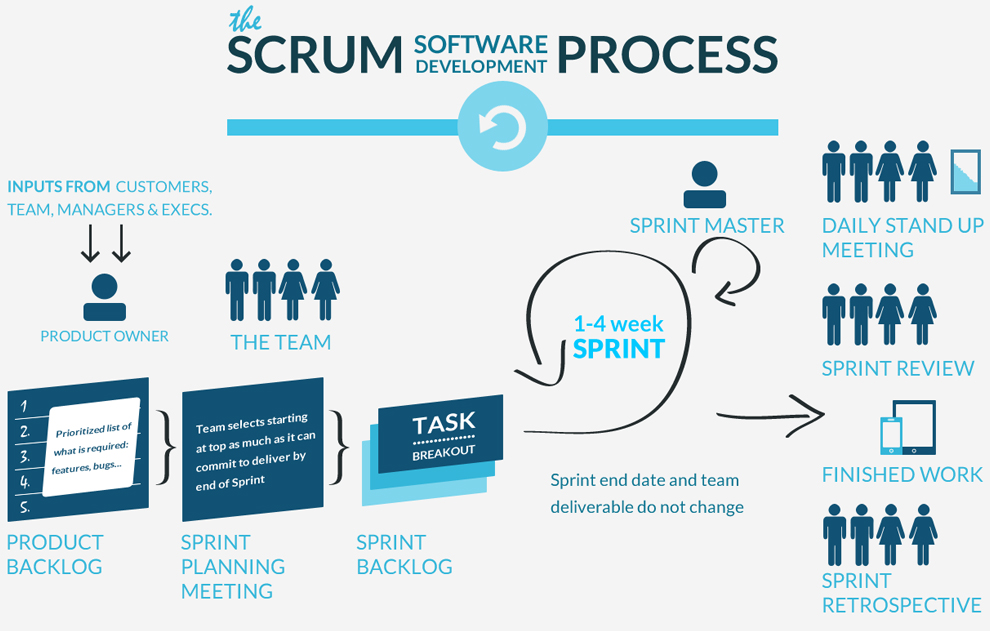
\includegraphics[width=0.9\textwidth]{scrumDevelopment}
    \caption{Scrum Software Development Process}
    \label{fig:waterfall}
\end{figure}

The process starts with the Product Catalog, where the product owner, which represents the stakeholders and customers, is responsible for understanding business and market requirements, and based on that creates a prioritized list of software requirements, and adds them to the Product Catalog. The Product owner maintains the Product Backlog up to date and at the quality level that the project team requires.

After that, a planning meeting is created, where the tasks for each sprint are identified in a form of Sprint Backlog and an estimated commitment for the sprint goal is made, followed by a review meeting, where the progress is reviewed and adjustments to be done in the next sprint are identified.

Each day during the sprint, the project team has a meeting, also called Daily Scrum, where each member gives feedback about what have been done since the last meeting, the current challenges and what is expected to be done until the next meeting.

Scrum is controlled by a Scrum Master, who is responsible for making the process run smoothly, for removing obstacles that impact productivity, and for organizing and facilitating the critical meetings. 

At the end of a sprint, the team conducts a sprint review during which the team demonstrates the new functionality to the product owner or any other stakeholder who wishes to provide feedback that could influence the next sprint.
Another activity in scrum project management is the sprint retrospective at the end of each sprint. The whole team participates in this meeting, including the Scrum Master and Product Owner. The meeting is an opportunity to reflect on the sprint that has ended, and identify opportunities to improve \cite{agile:scrum}.

\subsubsection{Extreme Programming (XP)}

is a software development methodology whose main goal is to improve software quality and responsiveness to changing customer requirements. 
XP uses an object-oriented approach as its paradigm of
drawing. The process consists of four activities: Planning, Project,
Encoding and Testing, which are repeated iterating through iteration.
Planning: It is created by the client, a set of stories that
Describe features and functionalities necessary for the software to be
built. Each story gives input to the methodology control system and is
Indexed and the client assigns it a priority value. Team members
Analyze this list and assign it costs if the story requires more than three
The client is asked to divide it. New stories can be added
any time. The next step is the team in collaboration with the customer
Decide which stories will get ready in the next iteration and on what date.
Project: The inherent philosophy is KIS (keep it simple), it is discouraged
Extra functionality because the developer
Thinks that later should be accurate. Often prototypes are generated,
Part of the project or of the whole. XP encourages
Refraction, a construction / design technique. (It is the process of changing and
Improve the internal software system, without altering the behavior
external.)
Encoding: Before the code, it recommends the process, that a
Battery of unit tests so that the story is satisfied. Then the focus of the
Programmers is the satisfaction of these unit tests. For coding XP,
Recommends that it be done in pairs. (Two heads work better than
), This guarantees other aspects such as quality, and speed (there is some
Scientific work that bought it to work in pairs, does not
Referring to Fig.
Yield, on the contrary usually more productivity is achieved).
Test: Unit tests are maintained over the various iterations and
Become part of a battery of regression tests, which is no longer
That all unit tests grouped together to be periodically tested for
Once in short periods (can be hours, at the end of the day, end of the week).
The idea is to confirm that nothing has stopped working.


blkabajkdkhakjsajdadads

\subsubsection{Feature Driven Development ( FDD )}
\subsubsection{Dynamic Systems Development Method ( DSDM) }
-------------------\\



Pros of Agile methods

Working software is delivered much more quickly and successive iterations can be delivered frequently, at a consistent pace.
There is closer collaboration between developers and the business.
Changes to requirements can be incorporated at any point of the process – even late in development.
It gives the opportunity for continuous improvement for live systems
It is highly transparent

Cons of Agile methods

Agile methodologies (e.g. Scrum, XP, Kanban, Crystal etc) are often more difficult to understand than linear, sequential ones – at least initially.
Because of the emphasis on working software there can be a perception that documentation can sometimes be neglected. The focus should be on appropriate documentation to the audience that needs it but, if not implemented well, this isn’t always the case.
When implemented badly Agile can introduce extra inefficiencies in large organisations or can be working against long standing organisational processes.

